\documentclass[dvipdfmx]{standalone}

\usepackage{color}
\usepackage{xcolor}
\usepackage{tikz}
\usepackage{pgfplots}
\usepackage{ifthen}
\usepackage{fp}

\usetikzlibrary{calc}

\def\startpoint{0}
\def\endpoint{1}

\newcounter{redplot}
\newcounter{blueplot}
\setcounter{redplot}{0}
\setcounter{blueplot}{0}

\newcount\input

\FPseed = \time

\message{プロット点数を入力してください}
\read-1 to \input

\begin{document}
  \scalebox{5}{
  % 描画する関数を決める
  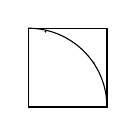
\begin{tikzpicture}[declare function = {func(\x) = sqrt(1-\x^2);}]
    % 枠を描画
    \draw (\startpoint,\startpoint) rectangle (\endpoint,\endpoint);
    % 関数を描画
    \draw plot[domain=\startpoint:\endpoint,samples=100] (\x,{func(\x)});
    \foreach \i in {1,...,\input}
    {
      % ランダムにx座標を決める
      \FPrandom{\randomX}
      \FPpow{\randomFuncX}{\randomX}{2}
      \FPsub{\randomFuncX}{1}{\randomFuncX}
      \FProot{\randomFuncX}{\randomFuncX}{2}
      \FPeval\plotX{\randomX}
      \FPeval\evalX{\randomFuncX}
      % ランダムにy座標を決める
      \FPrandom{\randomY}
      \FPeval\plotY{\randomY}
      % 関数の求める面積の内側の場合は赤,外側の場合は青で点をプロット
      % 赤の点と青の点を数える
      \pgfmathparse{\evalX > \plotY ? "blue" : "red"}
      \edef\color{\pgfmathresult}
      \ifthenelse{\equal{\color}{red}}{\stepcounter{redplot}}{\stepcounter{blueplot}}
      % 点をプロットする
      \filldraw[fill=\color, ultra thin] (\plotX, \plotY) circle [radius=(\endpoint-\startpoint)*0.01];
    }
  \end{tikzpicture}
  }
  % 枠内全体の面積を変数に代入
  \FPeval\overallS{\startpoint}
  % 点の比と面積の比の方程式を解き,面積の近似解を得る
  \FPeval\result{round(4 * \arabic{blueplot} * \overallS / \input,9)}
  \begin{tikzpicture}
    \draw (7,5) node {全体の点数 = \input};
    \draw (7,4) node {青い点数 = \arabic{blueplot}};
    \draw (7,3) node {赤い点数 = \arabic{redplot}};
    \draw (7,2) node {全体的な面積 = \overallS};
    \draw (7,1) node {$\displaystyle\int^1_0 4\sqrt{1-x^2}$ = \result};
  \end{tikzpicture}
\end{document}
